%%%%%%%%%%%%%%%%%%%%%%%%%%%%%%%%%%%%%%%%%%%%%%%%%%%%%
%		INTRODUCCION
%%%%%%%%%%%%%%%%%%%%%%%%%%%%%%%%%%%%%%%%%%%%%%%%%%%%%

\section[Introducci\'on]{Introducci\'on}
\subsection{Vidrios Met\'alicos}

\tikzstyle{every picture}+=[remember picture]

\begin{frame}
\frametitle{Vidrios Met\'alicos (Metal Amorfo)}

\tikzstyle{na} = [baseline=-.5ex]

\centering
\tikz[baseline]{\node[fill=gray!20,anchor=base] (t1){Vidrio};} \tikz[baseline]{\node[fill=gray!20,anchor=base] (t2){Met\'alico};}

\vspace{0.2cm}

\begin{columns}
  \begin{column}{0.48\paperwidth}
    \tikz[na]{\node[coordinate] (n1){};}
    \centering
    \begin{block}{Vidrio}
      \centering Estructura amorfa
      
      \vspace{0.2cm}
      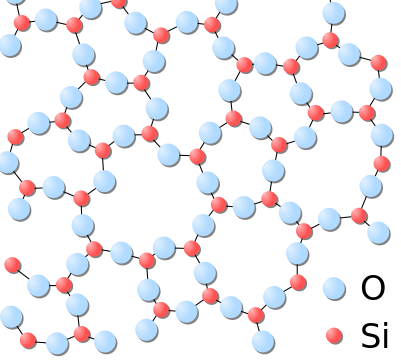
\includegraphics[width=3cm]{Cap_1/500px-Silica.png}
    \end{block}
  \end{column}
  \begin{column}{0.48\paperwidth}
    \tikz[na]{\node[coordinate] (n2) {};}
    \centering
    \begin{block}{Met\'alico}
      \centering Aleaci\'on met\'alica:\\
      Cu, Ni, Fe, Au, Zr, Be, La, Pd, Ti\\
      
      \vspace{0.2cm}
      Aunque tambi\'en puede contener no metales en baja concentraci\'on
    \end{block}
  \end{column}
\end{columns}

\begin{tikzpicture}[overlay]
        \path[->] (t1) edge [bend right] (n1);
        \path[->] (t2) edge [bend left] (n2);
\end{tikzpicture}

% \item Sus propiedades sobresalientes los hacen candidatos para aplicaciones modernas y de alta tecnolog\'ia. Material avanzado
\end{frame}

\definecolor{goodTitle}{HTML}{4D9A63}
\definecolor{goodDesc}{HTML}{A0DB8E}
\definecolor{alertTitle}{HTML}{FF2222}
\definecolor{alertDesc}{HTML}{FF9090}

\newcommand{\defaultBlocks}{
  \setbeamercolor{block title}{fg=white, bg=hsrmWarmGreyDark}
  \setbeamercolor{block body}{parent=palette secondary}
  \setbeamercolor{block title example}{fg=white, bg=hsrmSec1Dark}
  \setbeamercolor{block body example}{fg=white, bg=hsrmSec1}
  \setbeamercolor{block title alerted}{fg=white, bg=hsrmRedDark}
  \setbeamercolor{block body alerted}{fg=white, bg=hsrmRed}
}

\newcommand{\ventaja}[2]{
  \setbeamercolor{block title}{bg=goodTitle,fg=white}%
  \setbeamercolor{block body}{bg=goodDesc,fg=black}%
  \only<#1>{
    \begin{block}{Ventaja}%
    #2
    \end{block}%
   }
  \defaultBlocks%
}

\newcommand{\desventaja}[2]{
  \setbeamercolor{block title}{bg=alertTitle,fg=white}%
  \setbeamercolor{block body}{bg=alertDesc,fg=black}%
  \only<#1>{
    \begin{block}<#1>{Desventaja}%
    #2
    \end{block}%
  }
  \defaultBlocks%
}


\begin{frame}
\frametitle{Propiedades}
\begin{block}{¿Por qu\'e atrae el inter\'es de investigadores?}
 Combina propiedades de cer\'amicas y de metales a escala nanom\'etrica, resultando en un material de propiedades \'unicas
\end{block}
 
\ventaja{1}{{\begin{itemize}
             \item Alta dureza
             \item Resistencia al desgaste y la abrasi\'on
             \item Gran resistencia mec\'anica
             \item Alta resiliencia
            \end{itemize}
            }}

\end{frame}

\begin{frame}
\frametitle{Propiedades} 

\ventaja{1}{{\begin{itemize}
             \item Ausencia de efectos adversos debidos a fronteras de granos (resistencia a la corrosi\'on)
            \end{itemize}
            }}
\desventaja{1}{{\begin{itemize}
		\item Alto costo y grandes limitaciones de fabricaci\'on
		\item Gran p\'erdida de ductilidad ante la aparici\'on de bandas de corte
	      \end{itemize}
	      }}
            
\end{frame}

\begin{frame}
 \frametitle{Producci\'on}
 \vspace{-0.15cm}
 \begin{block}{}
    \textit{Te\'oricamente, todo l\'iquido podr\'ia convertirse en vidrio a velocidades de enfriamiento suficientemente altas y temperaturas suficientemente bajas evitando el proceso de cristalizaci\'on} \cite{turnbull61}
 \end{block}
 
 %Las t\'ecnicas de fabricaci\'on act\'uan sobre la composici\'on, el volumen y la velocidad de enfriamiento
 \begin{textblock*}{10cm}(1.4cm,4.9cm)
  \begin{columns}
    \begin{column}{4cm}
      \begin{figure}
	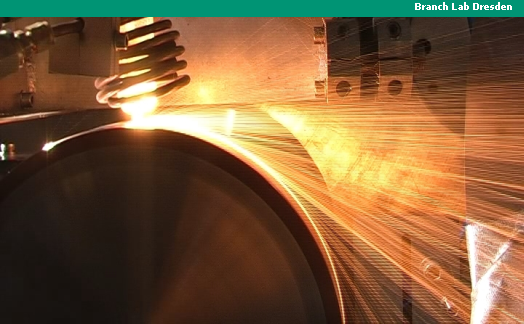
\includegraphics[width=4cm]{Cap_1/melt_spinning_B.png}
      \end{figure} 
      \begin{textblock*}{4cm}(1.3cm,8cm)
	\scriptsize{Proceso de \textit{Melt Spinnning}}
      \end{textblock*}
    \end{column}
    \begin{column}{6cm}
    \begin{alertblock}{Espesor}
	El espesor es un limitante. Los vidrios met\'alicos volum\'etricos, o \textit{Bulk Metallic Glasses} en ingl\'es, tienen una secci\'on transversal de por lo menos algunos mil\'imetros
    \end{alertblock}
    \end{column}
  \end{columns}
 \end{textblock*}
 
\end{frame}


\begin{frame}
 \frametitle{Aplicaciones}
 \centering
 Se trata de un material avanzado de ingenier\'ia
 
 
 \begin{figure}
 \centering
 \begin{tabularx}{\textwidth}{ccc}
 \only<1>{
 \subfloat[Filo est\'andar]{
    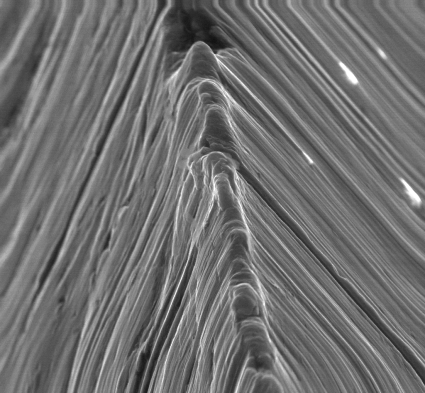
\includegraphics[width=3cm]{Cap_1/blade.png}}
  &
  \subfloat[Filo de BMG]{
    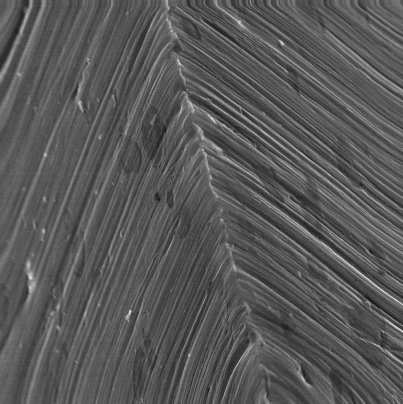
\includegraphics[width=3cm]{Cap_1/BMG-blade.png}}
  &
  \subfloat[Joyer\'ia]{
    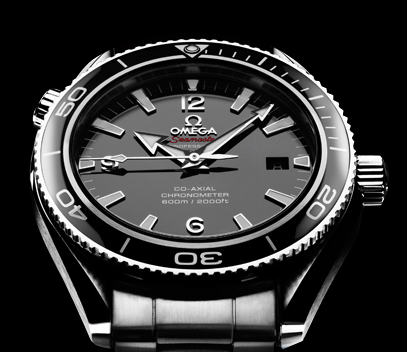
\includegraphics[width=3cm]{Cap_1/seamaster.png}}
  }
  \only<2>{
  \subfloat[Deportes]{
    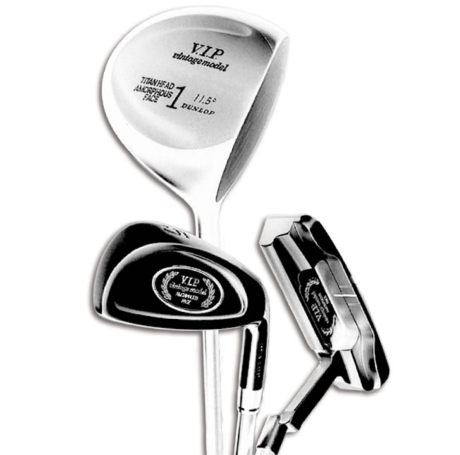
\includegraphics[width=3cm]{Cap_1/golf.png}}
  &
  \subfloat[MEMS]{
    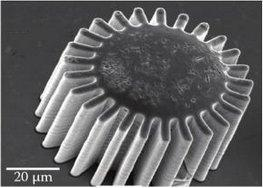
\includegraphics[width=3cm]{Cap_1/MEMS_A.jpeg}}
  &
  \subfloat[MEMS]{
    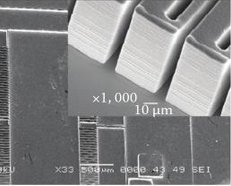
\includegraphics[width=3cm]{Cap_1/MEMS_B.jpeg}}
    }
 \end{tabularx}
\end{figure}
\end{frame}

\begin{frame}
 \frametitle{Mec\'anica de deformaci\'on}
 \begin{block}{Bandas de corte}
 Concentraci\'on de deformaci\'on en bandas estrechas, llamadas \textbf{bandas de corte}.
 El crecimiento de estas bandas puede causar la fractura fr\'agil del material \cite{schuh07}.
 \end{block}
 \begin{figure}
 \centering
 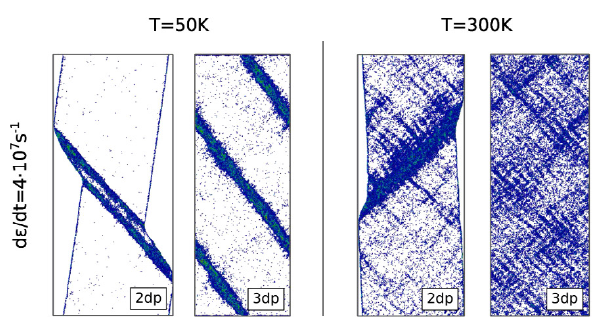
\includegraphics[width=5cm]{Cap_1/shearbands.png}
\end{figure}
\begin{textblock*}{\textwidth}(1cm,8.7cm)
 \centering
 \scriptsize{Muestra de BMG bajo tracci\'on uniaxial. Adaptado de \cite{albe13}}
\end{textblock*}

\end{frame}

\begin{frame}
 \frametitle{Objetivos}
 \vspace{0.5cm}
\begin{itemize}
 \item Investigar el comportamiento en r\'egimen elasto-pl\'astico en grandes deformaciones de un metal amorfo binario a diferentes temperaturas
 \begin{itemize}
  \item Estudiar el comportamiento de las \textbf{bandas de corte} y buscar posibles soluciones para evitar o retardar la falla fr\'agil
 \end{itemize}
 \item Investigar los efectos de cambios en la composici\'on sobre las propiedades mec\'anicas
 \begin{itemize}
  \item Generar muestras modificadas: porosidad variable e inclusiones cristalinas
 \end{itemize}
\end{itemize}
\end{frame}

